\subsection{Introduction to Functions}
To talk about functions, is to talk about \textbf{relationships}. Take the `<' sign, this
is a relationship. $x < y$ means $x$ relates to $y$, such that $x$ is less than $y$.\\

\noindent
\begin{center}
    Let $a=\{1,2,3,4\}$, $b=\{0,1,2,3\}$. Let $R$ be the relation `<', $aRb$ yields:
\end{center}

\vspace{1em}
\begin{figure}[ht]
    \centering
    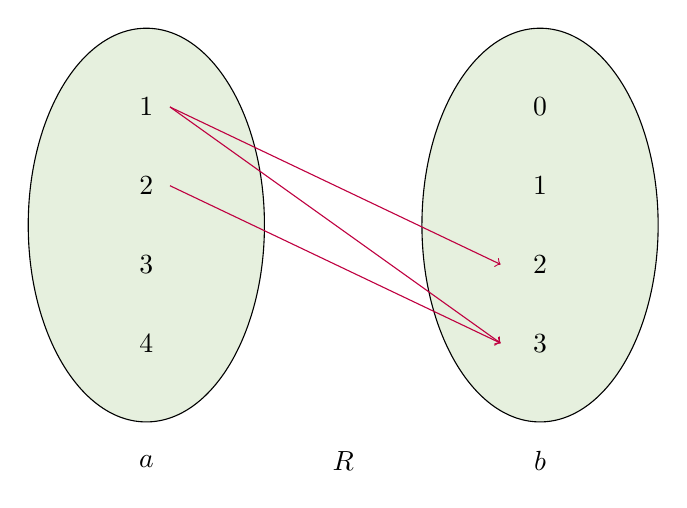
\begin{tikzpicture}
        % Draw the sets
        \draw[black, fill=OliveGreen!10] (-3,0) ellipse (1.5 and 2.5);
        \draw[black, fill=OliveGreen!10] (2,0) ellipse (1.5 and 2.5);


        % Labels for the elements in the first set
        \node at (-3,1.5) {1};
        \node at (-3,.5) {2};
        \node at (-3,-.5) {3};
        \node at (-3,-1.5) {4};
        \node at (-3,-3) {$a$};

        % Labels for the elements in the second set
        \node at (2,1.5) {0};
        \node at (2,.5) {1};
        \node at (2,-.5) {2};
        \node at (2,-1.5) {3};
        \node at (2,-3) {$b$};

        \node at (-.5,-3) {$R$};

        % Draw the arrow
        %1
        \draw[->, purple] (-2.7,1.5) -- (1.5,-.5);
        \draw[->, purple] (-2.7,1.5) -- (1.5,-1.5);

        %2
        \draw[->, purple] (-2.7,.5) -- (1.5,-1.5);
    \end{tikzpicture}
    \caption{\centering $R$ produces ordered pairs $\{(1,2),(1,3),(2,3)\}$, as $1<2$, $1<3$, $2<3$}.
    \label{fig:relates}
\end{figure}

\begin{Def}[Relation]{thm:relation}
    A relation $R$ on sets $a$ and $b$, $aRb$, is a subset of $a\times b$.
\end{Def}

\noindent
Since $a\times b$ is the set of all possible ordered pairs. $R$'s pairings must contain some or
all pairing of $a\times b$. This includes no pairing at all, the emptyset.\\

\noindent
The arrows in \textbf{Figure \ref{fig:relates}} are often referred to as \underline{\textbf{mappings}}. 1 maps to 2, 1 maps to 3, and 2 maps to 3.\\

\begin{Tip}
    When looking at Definitions, come up with examples on your own. The ability to explain a concept to someone else
    proves understanding.\\
\end{Tip}

\newpage


\begin{figure}
    Functions are a type of relation, where \underline{\textbf{each input has exactly one output.}}\\
    We can visualize this as a machine:\\\\


    \hspace{3em}
    \begin{tikzpicture}
        \node[label={below:{input}}] (A) at (3,0) {$x$};
        \pic (B) at (7,0) {machine={$f$}};
        \node[label={below:{output}}] (C) at (11,0) {$f(x)$};

        \draw[purple, -stealth] (A) -- (B-in);
        \draw[purple, -stealth] (B-out) -- (C);

    \end{tikzpicture}
    \caption{\centering The machine $f$ takes an input $x$ and produces an output $f(x)$.}
    \label{fig:machine}
\end{figure}

\noindent
In our previous example we used `<' as a relation. This is not a function, as\\
$1$ relates to $2$ and $3$. Instead let's use the absolute function, $f(x)=|x|$.

\begin{figure}[ht]
    \centering
    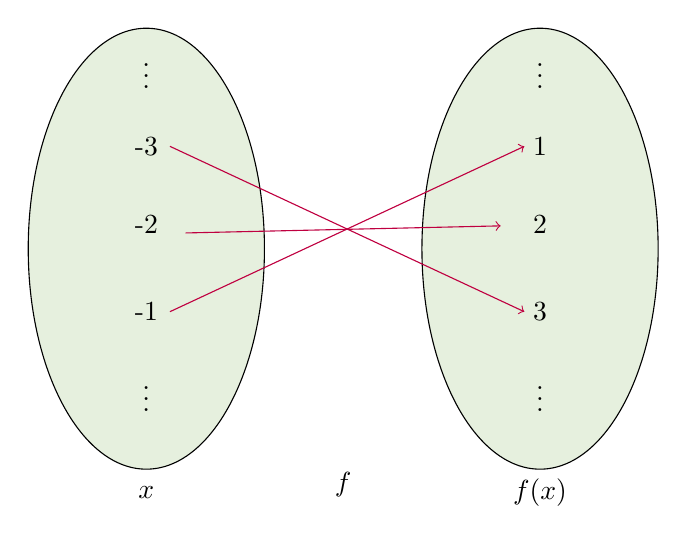
\begin{tikzpicture}
        % Draw the sets
        \draw[black, fill=OliveGreen!10] (-3,0) ellipse (1.5 and 2.8);
        \draw[black, fill=OliveGreen!10] (2,0) ellipse (1.5 and 2.8);


        % Labels for the elements in the first set
        \node at (-3,2.3) {\vdots};
        \node at (-3,1.3) {-3};
        \node at (-3,.3) {-2};
        \node at (-3,-.8) {-1};
        \node at (-3,-1.8) {\vdots};
        \node at (-3,-3.1) {$x$};

        % Labels for the elements in the second set
        \node at (2,2.3) {\vdots};
        \node at (2,1.3) {1};
        \node at (2,.3) {2};
        \node at (2,-.8) {3};
        \node at (2,-1.8) {\vdots};
        \node at (2,-3.1) {$f(x)$};

        \node at (-.5,-3) {$f$};

        % Draw the arrow
        %-3
        \draw[->, purple] (-2.7,1.3) -- (1.8,-.8);
        %-2
        \draw[->, purple] (-2.5,.2) -- (1.5,.29);
        %-1
        \draw[->, purple] (-2.7,-.8) -- (1.8,1.3);
    \end{tikzpicture}
    \caption{\centering Pairs $\{(-3,3),(-2,2),(-1,1)\}$, as $f(-3)=3$, $f(-2)=2$, $f(-1)=1$}.
    \label{fig:relates}
\end{figure}

\begin{Note}
    \textbf{Note}: f(x)=|x| is where x hasn't been chosen yet, choose 3, f(-3)=|-3|=3.
\end{Note}

\noindent
In \textbf{Figure \ref{fig:relates}}, assume inputs are integers. Then the absolute functions maps to \\
integers, i.e., \underline{if I put in an integer, I get out an integer.} In the figure we\\
represent this by the two green ovals; The left (inputs), the right (outputs).\\

\noindent
Our inputs are called the \textbf{domain}, the outputs the \textbf{codomain},\\
and all the possible mappings the \textbf{range}.\\

\newpage

\begin{Def}[Function]{Def:function}
    A function $f$ is a relation between two sets, $A$ (the domain) and $B$ (the codomain),
    such that each element in $A$ is mapped to exactly one element
    in $B$. The set of all possible outputs of $f$ is called the range of $f$.
\end{Def}

\noindent
Say we create a function $f(x)$, which tells us if someone prefers cats or dogs.\\

\begin{center}
    Let $P=\{\text{``Lois"}, \text{``Pete"}, \text{``Stuart"}\}$, $Q=\{\text{"Cats"}, \text{"Dogs"}\}$.
\end{center}

\begin{figure}[ht]
    \centering
    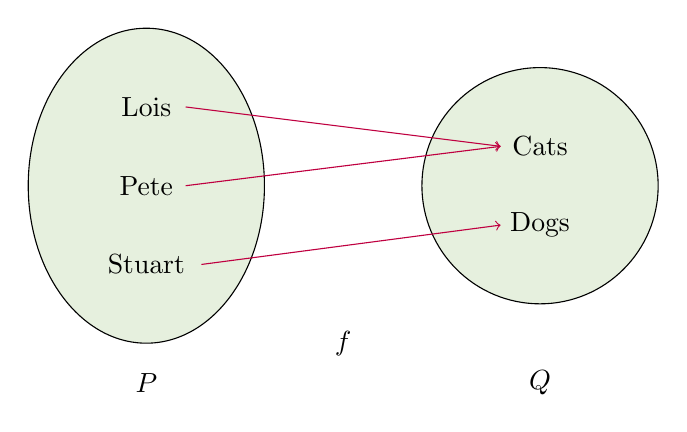
\begin{tikzpicture}
        % Draw the sets
        \draw[black, fill=OliveGreen!10] (-3,0) ellipse (1.5 and 2);
        \draw[black, fill=OliveGreen!10] (2,0) ellipse (1.5 and 1.5);


        % Labels for the elements in the first set
        \node at (-3,1) {Lois};
        \node at (-3,0) {Pete};
        \node at (-3,-1) {Stuart};
        \node at (-3,-2.5) {$P$};

        % Labels for the elements in the second set
        \node at (2,.5) {Cats};
        \node at (2,-.5) {Dogs};
        \node at (2,-2.5) {$Q$};

        \node at (-.5,-2) {$f$};

        % Draw the arrow
        %Lowis
        \draw[->, purple] (-2.5,1) -- (1.5,.5);
        %Peter
        \draw[->, purple] (-2.5,0) -- (1.5,.5);
        %Stewie
        \draw[->, purple] (-2.3,.-1) -- (1.5,-.5);
    \end{tikzpicture}
    \caption{\centering Produced ordered pairs $\{(\text{Lois},\text{Cats}),(\text{Pete},\text{Cats}),(\text{Stuart},\text{Dogs})\}$.}
    \label{fig:cats_dogs}
\end{figure}

\noindent
In function $f$, \underline{all elements in our domain map to an element in our
    codomain.} This makes our function \textbf{onto}, or \textbf{surjective}.\\

\begin{Def}[Onto (Surjective)]{thm:onto}
    A function $f$ is onto if every element in the codomain is mapped to by some element in the domain.
\end{Def}

\begin{graybox}
    \textbf{Comments:} Unrelated, take a break, stretch, get water. We sit down way
    too much. Taking a break doesn't mean consuming media, it means sitting with yourself, taking a walk.
    Work smart not hard, that means taking care of yourself. Having dedicated study time for x hours of your day
    with frequent breaks is great. Dedicating the entire day or all your free-time, not so much, you'll burnout in
    that very session or the next. Consistent small chunks always outpaces the cram, and it's a lot less stressful too.
    \vspace{-.2em}
\end{graybox}

\noindent
Now say we have a function $g(x)$, which tells us a person's student ID.\\
\begin{center}
    Let $T=\{\text{``Raven"}, \text{``Stella"}, \text{``Robbert"}\}$, $U=\{\text{"U001"}, \text{"U002"}, \text{U003}, ...\}$.
\end{center}

\begin{figure}[ht]
    \centering
    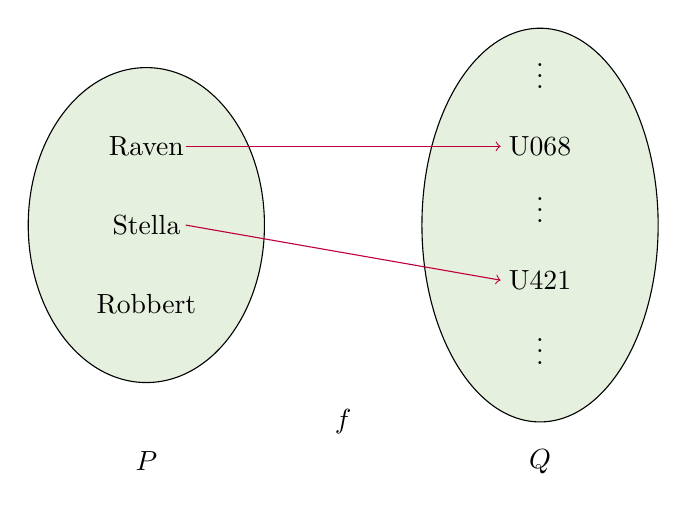
\begin{tikzpicture}
        % Draw the sets
        \draw[black, fill=OliveGreen!10] (-3,0) ellipse (1.5 and 2);
        \draw[black, fill=OliveGreen!10] (2,0) ellipse (1.5 and 2.5);


        % Labels for the elements in the first set
        \node at (-3,1) {Raven};
        \node at (-3,0) {Stella};
        \node at (-3,-1) {Robbert};
        \node at (-3,-3) {$P$};

        % Labels for the elements in the second set
        \node at (2, 2) {\vdots};
        \node at (2, 1) {U068};
        \node at (2,.3) {\vdots};
        \node at (2,-.7) {U421};
        \node at (2,-1.5) {\vdots};
        \node at (2,-3) {$Q$};

        \node at (-.5,-2.5) {$f$};

        % Draw the arrow
        %Raven
        \draw[->, purple] (-2.5,1) -- (1.5,1);
        %Stella
        \draw[->, purple] (-2.5,0) -- (1.5,-.7);
    \end{tikzpicture}
    \caption{\centering Produced ordered pairs $\{(\text{Raven},\text{U068}),(\text{Stella},\text{U421})\}$.
        not all elements have a mapping, meaning it is \textbf{not onto}.}
    \label{fig:cats_dogs}
\end{figure}

\noindent
In our example this suggests that ``Robbert" is not a registered student.\\

\noindent
\underline{Each element in the domain maps to exactly one element in the codomain.}\\
This makes our function \textbf{one-to-one}, or \textbf{injective}.\\

\begin{Def}[One-to-One (Injective)]{thm:one_to_one}
    A function $f$ is one-to-one if each element in the domain is mapped to exactly one element in the codomain.
\end{Def}

\noindent
If we were to change the function $g$, restricting the domain to only include
registered students, then our function would be \textbf{onto} and \textbf{one-to-one}. Since
each student has a unique ID, and each ID belongs to a student.\\

\noindent
When a function is both onto and one-to-one, it is called a \textbf{bijection}.\\

\begin{Def}[Bijection]{thm:bijection}
    A function $f$ is a bijection if it is both onto and one-to-one.
\end{Def}

\newpage